\chapter{Programmazione dinamica}
\section{Introduzione}
Finora, l'unica tecnica di risoluzione di problemi, o di ricerca di algoritmi,
che abbiamo visto è il \nameref{chap:divide-et-impera}. La \emph{programmazione
dinamica} è un'altra tecnica basata su un approccio molto simile.

Entrambe prevedono di spezzare il problema di partenza in sotto-problemi più
semplici e di ricostruire la soluzione del problema originale a partire dalle
soluzioni dei sotto-problemi. La differenza fondamentale sta nel fatto che la
\emph{programmazione dinamica} risolve ogni sotto-problema una sola volta,
mentre il \emph{Divide-et-impera} non pone questo vincolo.

Per realizzare ciò, le soluzioni di tutti i sotto-problemi vengono salvate in
una tabella che viene consultata ogni volta che è necessario risolvere uno
dei sotto-problemi. In particolare, se la tabella non contiene la soluzione
al sotto-problema considerato, questa viene calcolata e aggiunta alla tabella.
In caso contrario, viene sfruttata la soluzione già nota.

\subsection{Approccio generale}
\begin{figure}[hb!]
    \centering
    \scalebox{0.83}{
        \begin{graph}
            \tikzset{rect/.style={draw, rectangle, minimum size=15mm,
                rounded corners=0.25cm, inner sep=5mm}}
            \node[rect] (1) {Problema di ottimizzazione};
    
            \node[rect] (2) [below of=1, yshift=-7.5mm] {\shortstack{Definizione della soluzione\\in maniera ricorsiva}};
            \node[rect] (3) [right of=2, xshift=100mm] {\shortstack{Definizione del valore della\\soluzione in maniera ricorsiva}};
            \node[rect] (4) [above of=3, yshift=7.5mm] {Problema di conteggio};
    
            \node[rect] (5) [below of=3, xshift=-120mm, yshift=-15mm]
                {\emph{Divide-et-impera}};
            \node[rect] (6) [below of=3, xshift=-60mm, yshift=-15mm]
                {\emph{\shortstack{Programmazione\\dinamica}}};
            \node[rect] (7) [below of=3, xshift=0mm, yshift=-15mm]
                {\emph{Memoization}};
    
            \node[rect] (8) [below of=7, yshift=-7.5mm, xshift=-27.5mm]
                {Tabella delle soluzioni};

            \node[rect] (9) [right of=8, xshift=30mm] {\shortstack{Output\\numerico}};
            \node[rect] (10) [left of=8, xshift=-40mm]
                {\shortstack{Ricostruzione\\della soluzione}};
            \node[rect] (11) [left of=10, xshift=-30mm] {\shortstack{Soluzione\\ottima}};
    
            \path[->]   (1) edge (2)
                        (2) edge (3)
                        (4) edge (3)
                        (3.west)+(0mm, -2mm)
                            edge [bend right=15]
                            node [near end, left]
                                {\shortstack{Non ci sono sotto-problemi\\ripetuti}}
                        (5.north)
                        (3)
                            edge [bend right=5]
                            node [midway, left=2mm]
                                {\shortstack{Ci sono sotto-problemi\\ripetuti e devono essere\\ risolti tutti}}
                        (6)
                        (3)
                            edge [bend left=10]
                            node [midway, right]
                                {\shortstack{Ci sono sotto-problemi\\ripetuti, ma ne devono\\essere risolti solo\\alcuni}}
                        (7.north)
                        (6.south east)+(-1mm, 1mm) edge [bend left=15] (8)
                        (7.south west)+(1mm, 1mm) edge [bend right=15] (8)
                        (8) edge (9)
                        (8) edge (10)
                        (10) edge (11);
        \end{graph}
    }
    \caption{Schema generale di approccio}
\end{figure}\noindent
Lo schema di cui sopra mostra un approccio generale alla scelta della tecnica
risolutiva più adatta al tipo di problema da risolvere. In particolare,
distinguiamo la soluzione del problema dal proprio valore, ad esempio, nella
ricerca del \emph{cammino breve} tra due \emph{nodi}, la soluzione è il
\emph{cammino}, mentre il valore potrebbe esserne la lunghezza.

Una volta definiti questi parametri, se la suddivisione del problema non
porta a dover risolvere più volte uno stesso sotto-problema, possiamo procedere
ad implementare la soluzione sfruttando l'approccio \emph{Divide-et-impera}
classico. Caso contrario, ricadiamo nei casi d'uso della \emph{programmazione
dinamica}, ma dobbiamo ancora fare una distinzione: la risoluzione di alcuni dei
sotto-problemi potrebbe non essere necessaria per arrivare alla soluzione del
problema di partenza. Se il caso è questo, procediamo con la tecnica della
\emph{memoization} che non è altro se non un approccio top-down alla
\emph{programmazione dinamica} \q{classica}.

In ogni caso, utilizzando la \emph{programmazione dinamica} si arriva alla
definizione di una \emph{tabella delle soluzioni} e, se il problema è un
\emph{problema di conteggio}, da cui possiamo ricavare direttamente la soluzione.
Se invece stiamo considerando un \emph{problema di ottimizzazione}, la
soluzione dovrà essere ricavata attraverso un processo di \q{ricostruzione}.

\section{Gioco del domino}
Vediamo adesso un primo esempio di utilizzo della \emph{programmazione dinamica}
e di come la soluzione si differenzi, soprattutto in termini di efficienza, da
una classica soluzione \emph{divide-et-impera}.

\begin{problem}[Domino lineare]
    Il gioco del domino è basato su tessere di dimensione $2\times1$. Scrivere un
    algoritmo che prenda in input un valore intero positivo $n$ e restituisca il
    numero di modi in cui è possibile disporre le tessere del gioco in modo che
    creino un rettangolo $2\times n$.
\end{problem}\noindent
Ad esempio, per $n$ pari a 0, 1, 2, 3, 4 l'algoritmo dovrà restituire 1, 1,
2, 3, 5.
\begin{note}
    Per $n=0$, restituiamo 1 perché per ottenere un rettangolo di dimensione
    $2\times 0$ c'è un solo modo: non disporre nessuna tessera.
\end{note}\noindent
Basandoci sullo schema di cui sopra possiamo identificare questo problema con
un \emph{problema di conteggio} e quindi la prima cosa da fare è la \q{definizione
del valore della soluzione in maniera ricorsiva}.

\subsection{Approccio basato su divide-et-impera}

Chiamiamo $DP[n]$ la funzione che per ogni valore $n\in\mathbb{N}$ restituisce il
numero di disposizioni possibili delle tessere. La funzione $DP$ è ricorsiva, quindi,
prima di tutto identifichiamo il caso base: poiché per $n=0$ e $n=1$ $DP[n]=1$,
possiamo decidere che $DP[n]=1$ per $n\leq1$.

A questo punto, consideriamo il caso più complesso in cui dobbiamo esaminare un
rettangolo $2\times n$ arbitrariamente grande. Poiché le tessere del domino hanno
dimensione $2\times1$ e non posso essere posizionate in modo sfalsato, i
possibili posizionamenti di ogni tessera sono due: in verticale o in orizzontale.
Se ipotizzassimo di mettere una tessera verticale a destra o a sinistra del
rettangolo, il problema si ridurrebbe all'analisi di un rettangolo $2\times(n-1)$.
Se invece posizionassimo la tessera in orizzontale otterremmo una figura composta
da un rettangolo $2\times(n-2)$ e da un altro rettangolo più piccolo di
dimensione $1\times2$. Chiaramente, il rettangolo più piccolo corrisponde ad una
tessera orizzontale posta sopra o sotto quella che abbiamo già messo e, di
conseguenza, arriviamo alla conclusione che qual'ora si disponga una tessera in
orizzontale se ne debba sempre aggiungere anche una seconda sopra o sotto la prima.

\noindent
Fatta questa riflessione possiamo terminare dicendo che, dato un
generico rettangolo $2\times n$, il numero di possibili disposizioni di tessere
è pari a $DP[n-1]+DP[n-2]$ e che quindi la definizione della funzione ricorsiva
è:
\[DP[n]=\begin{cases}
    1 & n\leq1\\
    DP[n-1]+DP[n-2] & n>1
\end{cases}\]
\begin{note}
    Le soluzioni per $n-1$ e $n-2$ si sommano perché per ogni rettangolo $2\times
    n$ ho la possibilità di mettere una tessera verticale o due tessere orizzontali.
\end{note}

\bigskip\noindent
Provando a valutare la funzione per valori crescenti di $n$ otteniamo la
seguente sequenza:
\[1,1,2,3,5,8,13,21,34,55,89,\dots\]
che corrisponde esattamente alla \emph{sequenza di Fibonacci}. L'implementazione
dell'algoritmo corrisponde perciò all'implementazione della funzione per il
calcolo di tale sequenza.

\begin{minicode}{Prima implementazione della soluzione}
    \ind\bc{int} domino1(\bc{int} n)\\
        \indf if (n $\leq$ 1) then\\
            return 1\\
        \indf else\\
            return domino1(n-1) + domino1(n-2)
\end{minicode}\noindent
La \emph{funzione di ricorrenza} associata a questa funzione è la seguente:
\[T(n)=\begin{cases}
    1 & n\leq1\\
    T(n-1)+T(n-2) & n>1
\end{cases}\]
Per il \emph{\nameref{def:21}} la \emph{forma chiusa} di tale funzione è
$T(n)=\Theta(2^n)$. Un costo esponenziale è tutt'altro che efficiente, non
possiamo fare meglio di così?

\bigskip\noindent Proviamo ad esaminare l'\emph{albero delle invocazioni} per
$n=6$:

\begin{figure*}[h!]
\centering
\resizebox*{\linewidth}{!}{
\begin{graph}
    \node[main] (6-1)   {$6$};
    \node[main] (5-2)   [below left of=6-1, xshift=-35mm] {$5$};
    \node[main] (4-2)   [below right of=6-1, xshift=35mm] {$4$};

    \node[main] (4-3)   [below left of=5-2, xshift=-12.5mm] {$4$};
    \node[main] (3-3)   [below right of=5-2, xshift=12.5mm] {$3$};
    \node[main] (3-3d)  [below left of=4-2, xshift=-12.5mm] {$3$};
    \node[main] (2-3)   [below right of=4-2, xshift=12.5mm] {$2$};

    \node[main] (3-4)   [below left of=4-3] {$3$};
    \node[main] (2-4)   [below right of=4-3] {$2$};
    \node[main] (2-4d)  [below left of=3-3] {$2$};
    \node[main] (1-4)   [below right of=3-3] {$1$};
    \node[main] (2-4dd)   [below left of=3-3d] {$2$};
    \node[main] (1-4d)   [below right of=3-3d] {$1$};
    \node[main] (1-4dd)  [below left of=2-3] {$1$};
    \node[main] (0-4)   [below right of=2-3] {$0$};

    \node[main] (2-5)   [below of=3-4, xshift=-20] {$2$};
    \node[main] (1-5)   [below of=3-4, xshift=20] {$1$};
    \node[main] (1-5d)  [below of=2-4, xshift=-20] {$1$};
    \node[main] (0-5)  [below of=2-4, xshift=20] {$0$};
    \node[main] (1-5dd)  [below of=2-4d, xshift=-20] {$1$};
    \node[main] (0-5d)  [below of=2-4d, xshift=20] {$0$};
    \node[main] (1-5ddd)  [below of=2-4dd, xshift=-20] {$1$};
    \node[main] (0-5dd)  [below of=2-4dd, xshift=20] {$0$};

    \node[main] (1-6) [below of=2-5, xshift=-15] {$1$};
    \node[main] (0-6) [below of=2-5, xshift=15] {$0$};

    \path[-]    (6-1) edge (5-2)
                (6-1) edge (4-2)
                (5-2) edge (4-3)
                (5-2) edge (3-3)
                (4-2) edge (3-3d)
                (4-2) edge (2-3)
                (4-3) edge (3-4)
                (4-3) edge (2-4)
                (3-3) edge (2-4d)
                (3-3) edge (1-4)
                (3-3d) edge (2-4dd)
                (3-3d) edge (1-4d)
                (2-3) edge (1-4dd)
                (2-3) edge (0-4)
                (3-4) edge (2-5)
                (3-4) edge (1-5)
                (2-4) edge (1-5d)
                (2-4) edge (0-5)
                (2-4d) edge (1-5dd)
                (2-4d) edge (0-5d)
                (2-4dd) edge (1-5ddd)
                (2-4dd) edge (0-5dd)
                (2-5) edge (1-6)
                (2-5) edge (0-6);
\end{graph}
}
\end{figure*}\noindent
Se ogni \emph{nodo} rappresenta un sotto-problema, è evidente come molti
sotto-problemi vengano risolti più di una volta. Questa è sicuramente
un'inefficienza, quindi, proviamo ad evitare di eseguire invocazioni ridondanti.

\subsection{Approccio basato su programmazione dinamica}
La presenza di sotto-problemi ripetuti ci costringe quindi ad evitare una
soluzione realizzata con un classico \emph{divide-et-impera}, e ad utilizzare
invece la \emph{programmazione dinamica}, con conseguente costruzione di una
\emph{tabella delle soluzioni}. In particolare, tale tabella conterrà un elemento
per ogni sotto-problema da risolvere.

Poiché, per ogni $n\in\mathbb{N}$ il calcolo della soluzione si basa su i due
valori precedenti di $n$, ci troviamo in una situazione in cui tutti i
sotto-problemi devono essere risolti e quindi procediamo con la
\emph{programmazione dinamica} classica o bottom-up. Ciò significa che per
costruire la \emph{tabella delle soluzioni} partiamo dai casi base e risaliamo
fino ad $n$.

\begin{minicode}{Seconda implementazione della soluzione}
    \ind\bc{int} domino2(\bc{int} n)\\
        \bc{int}[] DP = new \bc{int}[0\dots n]\hfill\com{\emph{Tabella delle soluzioni}}
        DP[0] = 1\\
        DP[1] = 1\\
        \indf for (i = 2 to n) do\\
            DP[i] = DP[i - 1] + DP[i - 2]\\
        \indf return DP[n]
\end{minicode}
\begin{note}
    Sebbene finora avessimo parlato soltanto di soluzioni ricorsive, nulla ci
    vieta di realizzarne di iterative se queste sono estensionalmente equivalenti.
\end{note}\noindent
L'aumento in efficienza è evidente in quanto la \emph{complessità} si è ridotta
a $\Theta(n)$, tuttavia, l'utilizzo di una \emph{tabella delle soluzioni} ci
porta a considerare anche la \emph{complessità} dal punto di vista spaziale, cioè
quanto spazio di memoria è necessario per la sua memorizzazione. In questo caso
memorizziamo i valori in un vettore di dimensione $n+1$, quindi la
\emph{complessità} è $S(n)=\Theta(n)$.

\bigskip\noindent Possiamo fare meglio di così?

Da un punto di vista temporale no, ma da quello spaziale si. Se consideriamo bene
la funzione ci rendiamo facilmente conto del fatto che, ad ogni iterazione,
utilizziamo soltanto i valori delle due posizioni precedenti. Di conseguenza,
potremmo eliminare il vettore e utilizzare delle semplici variabili.

\begin{minicode}{Terza implementazione della soluzione}
    \ind\bc{int} domino3(\bc{int} n)\\
        \bc{int} DP$_0$ = 1\\
        \bc{int} DP$_1$ = 1\\
        \bc{int} DP$_2$ = 1\\
        \indf for (i = 2 to n) do\\
            DP$_0$ = DP$_1$\\
            DP$_1$ = DP$_2$\\
            DP$_2$ = DP$_1$ + DP$_0$\\
        \indf return DP$_2$
\end{minicode}\noindent
Ora, la \emph{complessità spaziale} si è ridotta a $\Theta(1)$.

\paragraph{Criterio di costo logaritmico}
Le \emph{complessità} calcolate finora sono tali fino a quando ci basiamo su
un \emph{criterio di costo uniforme}, nel quale consideriamo soltanto il
numero di elementi. Ora però, proviamo a chiederci come cambierebbero le
\emph{complessità} se utilizzassimo un \emph{criterio di costo logaritmico}.

\noindent
Iniziamo ragionando sul modo in cui crescono i numeri della serie di Fibonacci.
Se $F(n)$ è l'$n$-esimo numero della serie, vale la \emph{formula di Binet}:
\[F(n)=\frac{\phi^n}{\sqrt{5}}-\frac{(1-\phi)^n}{\sqrt{5}}\quad\text{con}
\quad\phi=\frac{1+\sqrt{5}}{2}=1.6180339887\dots\footnotemark\]
\begin{note}
    Vale la pena far notare che $F(n)=DP[n-1]$ perché $DP$ vale per $n\geq0$,
    mentre $F(n)$ per $n\geq1$.
\end{note}\noindent
Il primo termine della formula è un'esponenziale con base un numero maggiore di $1$,
quindi cresce esponenzialmente, mentre il secondo tende a $0$. Questo ci dice
che i bit necessari a memorizzare l'$n$-esimo valore della serie crescono
linearmente. Ovvero, per memorizzare l'$n$-esimo termine servono $\Theta(n)$ bit
e sommare due valori consecutivi costa $\Theta(n)$.

\footnotetext{$\phi$ rappresenta il valore della \emph{sezione aurea} ed è
anche definito come $\lim_{n\to+\infty}\frac{F(n+1)}{F(n)}$, ovvero come
il rapporto tra numeri consecutivi della serie di Fibonacci}

Detto questo, possiamo ricalcolare tutte le \emph{complessità} delle tre soluzioni
sotto il \emph{criterio di costo logaritmico}.

\begin{table}[h!]
    \centering
    \renewcommand{\arraystretch}{1.2}
    \begin{tabular}{|c|c|c|}
        \hline
        \textbf{Soluzione} & \textbf{Complessità temporale} & \textbf{Complessità
        spaziale} \\
        \hline
        \texttt{domino1} & $O(n2^n)$ & $O(n^2)$\\
        \hline
        \texttt{domino2} & $O(n^2)$ & $O(n^2)$\\
        \hline
        \texttt{domino3} & $O(n^2)$ & $O(n)$\\
        \hline
    \end{tabular}
\end{table}
\begin{note}
    In pratica, abbiamo semplicemente moltiplicato per $n$ tutti i valori.
\end{note}

\section{Problema di Hateville}
\begin{problem}[Hateville]
    Hateville è un villaggio particolare composto da $n$ case numerate e
    disposte linearmente lungo una singola strada. Ad Hateville ognuno odia i
    propri vicini: l'abitante $i$ odia i suoi vicini $i-1$ e $i+1$ (se esistono).

    Si vuole realizzare una sagra per la quale è necessario raccogliere dei fondi.
    Ogni abitante $i$ è disposto a donare una quantità $D[i]$, ma solo se nessuno
    dei suoi vicini partecipa.

    Scrivere un algoritmo che restituisca la quantità massima di fondi che può
    essere raccolta e un secondo algoritmo che restituisca il sottoinsieme di
    indici $S\subseteq\{1,\dots,n\}$ tale per cui la donazione totale $T=\sum_{i
    \in S}D[i]$ sia massimale.
\end{problem}\noindent
Ad esempio, se il vettore delle donazioni è $D=[10,5,5,10]$ la massima quantità
di fondi che può essere raccolta è $20$ e l'insieme $S$ è $\{1,4\}$.

\subsection{Approccio basato su divide-et-impera}
Iniziamo provando a ridefinire il problema. Se $HV(i)$ è uno dei possibili
insiemi di indici che consente di ottenere una raccolta massimale dalle prime
$i$ case, la soluzione al problema è $HV(n)$.

Consideriamo ora il vicino $i$. Possiamo accettare o meno la sua donazione.
Se non la accettiamo possiamo accettare quella del vicino $i-1$ e quindi
$HV(i)=HV(i-1)$. Se invece accettiamo la donazione di $i$, dobbiamo rifiutare
quella di $i-1$, perciò $HV(i)=HV(i-2)\cup\{i\}$.

\noindent
Per decidere se accettare o meno la donazione di $i$ è sufficiente vedere
quale scelta permette di raccogliere più fondi. Se $highest$ è una
funzione che, dati due insiemi, seleziona quello che garantisce una donazione
più alta, $HV(i)$ diventa:
\[HV(i)=highest\left(HV(i-1),HV(i-2)\cup\{i\}\right)\]
Ciò che abbiamo detto finora è vero secondo quanto affermato dal seguente teorema:
\begin{definition}[Sottostruttura ottima]
    Siano $P_i$ il problema dato dalle prime $i$ case e $S_i$ una sua soluzione
    ottima. Valgono le seguenti:
    \begin{enumerate}
        \item Se $i\notin S_i$, allora $S_i=S_{i-1}$;
        \item Se $i\in S_i$, allora $S_i=S_{i-2}\cup\{i\}$;
    \end{enumerate}
\end{definition}

\begin{proof}[Dimostrazione]
    Procediamo dimostrando separatamente i due punti.
    \paragraph{Caso 1: \bm{$i\notin S_i$}}
    Secondo il teorema, $S_i=S_{i-1}$, cioè $S_i$ è la soluzione ottima sia di
    $P_i$ che di $P_{i-1}$. Se supponessimo, per assurdo, che non fosse così,
    dovrebbe esistere una soluzione $S'_{i-1}$ per il problema $P_{i-1}$ tale
    che $S'_{i-1}=highest\left(S'_{i-1}, S_i\right)$. Cioè, la soluzione $S'_{i-1}$
    dovrebbe garantire una donazione maggiore di quella di $S_i$. Ma, se fosse
    così, $S'_{i-1}$ dovrebbe essere anche la soluzione di $P_i$, generando un
    assurdo.

    \paragraph{Caso 2: \bm{$i\in S_i$}}
    Se $i\in S_i$, $i-1\notin S_i$, altrimenti non sarebbe una soluzione
    ammissibile. Quindi, $S_i-\{i\}$ deve essere una soluzione ottima per
    $P_{i-2}$. Se supponessimo, per assurdo, che non fosse così, dovrebbe
    esistere una soluzione $S'_{i-2}$ per il problema $P_{i-2}$ tale che
    $S'_{i-2}=highest\left(S'_{i-2}, S_i-\{i\}\right)$. Ma, se fosse così,
    $S'_{i-2}\cup\{i\}$ dovrebbe essere una soluzione di $P_i$ migliore di
    $S_i$, generando un assurdo.
\end{proof}\noindent
Dimostrate le nostre ipotesi, possiamo procedere con la definizione ricorsiva
della soluzione. I casi base sono due:
\begin{itemize}
    \item Se $i=0$, $HV(0)=\emptyset$;
    \item Se $i=1$, $HV(1)=\{1\}$;
\end{itemize}
La funzione che otteniamo è la seguente:
\[HV(i)=\begin{cases}
    \emptyset & i=0\\
    \{1\} & i=1\\
    highest\left(HV(i-1), HV(i-2)\cup\{i\}\right) & i\geq2
\end{cases}\]
Osservando la definizione possiamo notare la similitudine con la funzione per il
calcolo della \emph{sequenza di Fibonacci}. Essendoci sotto-problemi ripetuti,
possiamo scartare subito qualunque soluzione basata su \emph{divide-et-impera}.

\subsection{Approccio basato su programmazione dinamica}
La \emph{programmazione dinamica} ci richiede di costruire una \emph{tabella
delle soluzioni}. Proviamo a costruire tale tabella partendo da un esempio:
sia il vettore delle donazioni $D$ definito come segue:
\[D=[10,5,5,8,4,7,12]\]

\newpage\noindent
La \emph{tabella delle soluzioni} è la seguente:

\begin{table}[ht!]
    \centering
    \renewcommand{\arraystretch}{1.2}
    \begin{tabular}{|c|c|c|c|c|c|c|c|c|}
        \hline
        \bm{$i$} & \bm{$0$} & \bm{$1$} & \bm{$2$} & \bm{$3$} & \bm{$4$} & 
        \bm{$5$} & \bm{$6$} & \bm{$7$}\\
        \hline
        $HV$ & $\emptyset$ & $\{1\}$ & $\{1\}$ & $\{1,3\}$ & $\{1,4\}$ &
        $\{1,3,5\}$ & $\{1,4,6\}$ & $\{1,3,5,7\}$\\
        \hline
    \end{tabular}
\end{table}\noindent
Ci sono un paio di problemi. Prima di tutto dobbiamo definire la funzione
$highest$, ma il problema più grosso è la difficoltà di memorizzazione degli
insiemi in una tabella.

Per risolvere entrambi i problemi in una volta potremmo definire il valore delle
soluzioni come la quantità di fondi che vengono raccolti. Definiamo quindi una
funzione $DP$ tale che $DP[i]$ è la massima quantità di fondi che si possono
ottenere dalle prime $i$ case di Hateville. Partendo da $HV$ possiamo definire
$DP$ come segue:
\[DP[i]=\begin{cases}
    0 & i=0\\
    D[1] & i=1\\
    \max\left(DP[i-1], DP[i-2]+D[i]\right) & i\geq2
\end{cases}\]\noindent
Adesso implementare la soluzione è una banalità.

\begin{minicode}{Implementazione della soluzione al primo problema}
\ind\bc{int} hateville(\bc{int}[] D, \bc{int} n)\\
    \bc{int}[] DP = new \bc{int}[0\dots n]\hfill\com{\emph{Tabella delle soluzioni}}
    DP[0] = 0\\
    DP[1] = D[1]\\
    \indf for (i = 2 to n) do\\
        DP[i] = max(DP[i - 1], DP[i - 2] + D[i])\\
    \indf return DP[n]
\end{minicode}\noindent
La \emph{complessità temporale} e \emph{spaziale} della soluzione sono entrambe
$\Theta(n)$. Possiamo notare che, come nel problema del domino, per ogni $i$ la
soluzione è ottenuta a partire dalle soluzioni dei due valori precedenti di $i$,
quindi, potremmo eliminare l'array e introdurre delle variabili semplici
riducendo a $\Theta(1)$ la \emph{complessità spaziale}.

\begin{minicode}{Implementazione migliorata della soluzione al primo problema}
\ind\bc{int} hateville(\bc{int}[] D, \bc{int} n)\\
    \bc{int} DP$_0$ = 0\\
    \bc{int} DP$_1$ = 1\\
    \bc{int} DP$_2$ = 1\\
    \indf for (i = 2 to n) do\\
        DP$_2$ = max(DP$_1$, DP$_0$ + D[i])\\
    \indf return DP$_2$
\end{minicode}

\paragraph{Ricostruire la soluzione}
A questo punto abbiamo risolto la prima richiesta del problema. Per quanto
riguarda la seconda, dobbiamo riuscire a ricostruire l'insieme di indici a
partire dalla \emph{tabella delle soluzioni}. Grazie al teorema sulla
\emph{\nameref{def:107}} possiamo fare le seguenti assunzioni:
\begin{itemize}
    \item Se la casa $i$ non è stata selezionata, $i\notin S_i$ e quindi $S_i=S_
    {i-1}$. Questo, riflesso sulla \emph{tabella delle soluzioni}, garantisce che
    se $DP[i]=DP[i-1]$, $i$ non appartiene all'insieme $S$ di indici;
    \item Se la casa $i$ è stata selezionata, $i\in S_i$ e quindi $S_i=S_{i-2}
    \cup\{i\}$. Questo, riflesso sulla \emph{tabella delle soluzioni}, garantisce
    che se $DP[i]=DP[i-2]+D[i]$, $i$ appartiene all'insieme $S$ di indici;
\end{itemize}
\begin{note}
    È possibile che risultino verificati entrambi i casi e, se succede, significa
    che esistono due soluzioni possibili.
\end{note}\noindent
Chiariti questi punti, possiamo ricostruire la soluzione fino a $i$ in modo
ricorsivo. Nello specifico, se $DP[i]=DP[i-1]$, si prende la soluzione valida per
$i-1$, altrimenti si prende quella valida per $i-2$ e le si aggiunge $i$.

\begin{minicode}{Implementazione della soluzione al secondo problema}
\ind\bc{SET} hateville(\bc{int}[] D, \bc{int} n)\\
    \bc{int}[] DP = new \bc{int}[0\dots n]\hfill\com{\emph{Tabella delle soluzioni}}
    DP[0] = 0\\
    DP[1] = D[1]\\
    \indf for (i = 2 to n) do\\
        DP[i] = max(DP[i - 1], DP[i - 2] + D[i])\\
    \indf return solution(DP, n)\\

\com{Funzione ausiliaria per la ricostruzione della soluzione}
\rmindent\ind\bc{SET} solution(\bc{int}[] DP, \bc{int} i)\\
    \indf if (i == 0) then\\
        return $\emptyset$\\
    \indf if (i == 1) then\\
        return \{1\}\\
    \indf if (DP[i] == DP[i - 1]) then\\
        return solution(DP, i - 1)\\
    \indf else\\
        \bc{SET} sol = solution(DP, i - 2)\\
        sol.insert(i)\\
        return sol\\
\end{minicode}\noindent
La \emph{complessità temporale} di \texttt{solution} è $\Theta(n)$.
\begin{note}
    È importante notare che non avremmo potuto ricostruire la soluzione senza
    l'intera \emph{tabella delle soluzioni} e quindi non possiamo utilizzare
    la versione migliorata di \texttt{hateville}.
\end{note}

\section{Problema dello zaino}
\begin{problem}[Problema dello zaino\footnotemark]
    Dato un insieme di oggetti, ognuno caratterizzato da un peso e da un profitto,
    e uno \q{zaino} di capacità finita, individuare un sottoinsieme di oggetti
    tali per cui il loro peso totale sia al più uguale alla capacità dello zaino
    e il loro profitto totale sia massimale.
\end{problem}

\footnotetext{Questo è uno dei problemi classici dell'informatica ed è noto
con il nome di \emph{Knapsack problem}}\noindent
Questo problema ci chiede di realizzare un algoritmo che prenda in input un
vettore $w$ dei pesi, un vettore $p$ dei profitti e la capacità $C$ dello zaino
e che restituisca un insieme $S\subseteq\{1,\dots,n\}$ tale che:
\begin{itemize}
    \item il peso totale non superi la capacità, cioè $w(S)=\sum_{i\in S}w[i]
    \leq C$;
    \item il profitto totale sia massimale, cioè $argmax_S\ p[S]=\sum_{i\in S}
    p[i]$;
\end{itemize}
Ad esempio, se $C=12$, $w=[10,4,8]$ e $p=[20,6,12]$, l'algoritmo deve
restituire l'insieme $S=\{1\}$.

\bigskip\noindent
Proviamo a dare un valore alla soluzione. Definiamo una funzione $DP[i][c]$ come
il massimo profitto che può essere ottenuto dai primi $0\leq i\leq n$ oggetti
in uno zaino di capacità $c\leq C$. Il massimo profitto ottenibile nel problema
originale è allora $DP[n][C]$.

Ora, consideriamo un generico oggetto $i$. Se non lo prendiamo, $DP[i][c]=
DP[i-1][c]$ perché non cambiano né il profitto né la capacità. Se invece lo
prendiamo, $DP[i][c]=DP[i-1][c-w[i]]+p[i]$ in quanto, il peso dell'oggetto $i$
viene sottratto alla capacità rimanente e il profitto associato viene aggiunto
a quello ottenuto con i precedenti $i-1$ oggetti.

La scelta migliore tra le due è quella che massimizza il profitto e la possiamo
sintetizzare con la seguente:
\[DP[i][c]=\max\left(\overbrace{DP[i-1][c-w[i]]+p[i]}^{\text{Preso}},\;
\overbrace{DP[i-1][c]}^{\text{Non preso}}\right)\]
Per quanto riguarda i casi base, è facile dedurre che per $i=0$ o $c=0$, il
profitto massimo possibile sia $0$. C'è però un terzo caso: quando proviamo a
prendere un oggetto, lo facciamo senza verificare che il peso non superi la
capacità, quindi, potremmo ritrovarci ad avere un valore negativo per quest'ultima.
Se questo succede, è ovvio che non avremmo potuto raccogliere quell'oggetto e,
di conseguenza, decidiamo che in quel caso il profitto valga $-\infty$ in modo da
assicurare che non venga selezionato dalla funzione $\max$.

Detto questo, possiamo scrivere la formula nella sua forma completa:
\[DP[i][c]=\begin{cases}
    0 & i=0 \vee c=0\\
    -\infty & c<0\\
    \max\left(DP[i-1][c-w[i]]+p[i],\; DP[i-1][c]\right) & \text{altrimenti}
\end{cases}\]
Equivalentemente, possiamo rimuovere il $-\infty$ e riscrivere la formula come
segue:
\[DP[i][c]=\begin{cases}
    0 & i=0 \vee c=0\\
    DP[i-1][c] & w[i]>c\\
    \max\left(DP[i-1][c-w[i]]+p[i],\; DP[i-1][c]\right) & w[i]\leq c
\end{cases}\]

\subsection{Approccio basato su programmazione dinamica}
\begin{minicode}{Implementazione iterativa della soluzione}
\ind\bc{int} knapsack(\bc{int}[] w, \bc{int}[] p, \bc{int} n, \bc{int} C)\\
    \bc{int}[][] DP = new \bc{int}[0\dots n][0\dots C]\hfill\com{\emph{Tabella
    delle soluzioni}}
    \indf for (i = 0 to n) do\\
        DP[i][0] = 0\\
    \indf for (c = 0 to C) do\\
        DP[0][c] = 0\\
    \indf for (i = 1 to n) do\\
        \indff for (c = 1 to C) do\\
            \indfff if (w[i] $\leq$ c) then\\
                DP[i][c] = max(DP[i - 1][c - w[i]] + p[i], DP[i - 1][c])\\
\end{minicode}
\begin{codecont}
    \indff else\\
        \indfff DP[i][c] = DP[i - 1][c]\\
    \rmindent return DP[n][C]
\end{codecont}

\begin{eg}[Esempio di esecuzione]
    Dato uno zaino di capacità $C=9$ e i seguenti vettori dei pesi e dei
    profitti:
    \[w=[4,2,3,4]\]
    \[p=[10,7,8,6]\]
    al termine dell'esecuzione dell'algoritmo di cui sopra, la matrice $DP$
    corrisponde alla seguente tabella:

    \begin{table}[h!]
        \renewcommand{\arraystretch}{1.2}
        \centering
        \begin{tabular}{|c|c|c|c|c|c|c|c|c|c|c|}
            \hline
             & \multicolumn{10}{c|}{\bm{$c$}}\\
            \hline
            \bm{$i$} & \bm{$0$} & \bm{$1$} & \bm{$2$} & \bm{$3$} & \bm{$4$} &
            \bm{$5$} & \bm{$6$} & \bm{$7$} & \bm{$8$} & \bm{$9$}\\
            \hline
            \bm{$0$} & 0 & 0 & 0 & 0 & 0 & 0 & 0 & 0 & 0 & 0\\
            \hline
            \bm{$1$} & 0 & 0 & 0 & 0 & 10 & 10 & 10 & 10 & 10 & 10\\
            \hline
            \bm{$2$} & 0 & 0 & 7 & 7 & 10 & 10 & 17 & 17 & 17 & 17\\
            \hline
            \bm{$3$} & 0 & 0 & 7 & 8 & 10 & 15 & 17 & 18 & 18 & 25\\
            \hline
            \bm{$4$} & 0 & 0 & 7 & 8 & 10 & 15 & 17 & 18 & 18 & 25\\
            \hline
        \end{tabular}
    \end{table}
\end{eg}

\paragraph{Complessità}
Siccome l'algoritmo costruisce e popola una tabella di dimensione $n\cdot C$,
la \emph{complessità} è $T(n)=\Theta(nC)$. Ovviamente lo stesso vale anche per 
la \emph{complessità spaziale}. Quindi, il costo dell'algoritmo dipende da due
variabili, ma poiché $C$ non rappresenta la dimensione dell'input e viene
rappresentato mediante $k=\lceil\log C\rceil$ bit, la \emph{complessità
temporale} può essere riscritta come:
\[T(n)=\Theta(n2^k)\]
Ciò, rende questa implementazione dell'algoritmo \emph{pseudo-polinomiale}\footnotemark.

\footnotetext{Parleremo meglio di cosa significhi più avanti nella trattazione}

\bigskip\noindent
È possibile fare meglio di così?

Possiamo provare a realizzare una versione ricorsiva dell'algoritmo.

\begin{minicode}{Implementazione ricorsiva della soluzione}
\ind\bc{int} knapsack(\bc{int}[] w, \bc{int}[] p, \bc{int} n, \bc{C})\\
    return knapsackRec(w, p, n, C)\\

\ind\bc{int} knapsackRec(\bc{int}[] w, \bc{int}[] p, \bc{int} n, \bc{c})\\
    \indf if (c $\leq$ 0) then\\
        return -$\infty$\\
    \indf if (i == 0 or c == 0) then\\
        return 0\\
    \indf\bc{int} notTaken = knapsackRec(w, p, i - 1, c)\\
    \indf\bc{int} taken = knapsackRec(w, p, i - 1, c - w[i]) + p[i]\\
    \indf return max(notTaken, taken)
\end{minicode}\noindent
In questa implementazione abbiamo semplicemente tradotto in codice la prima
forma della formula per $DP$ e l'\emph{equazione di ricorrenza} è:
\[T(n)=\begin{cases}
    1 & n\leq1\\
    2T(n-1)+1 & n>1
\end{cases}\]
Per il \emph{\nameref{def:21}} la \emph{forma chiusa} associata è
$T(n)=\Theta(2^n)$ e quindi la \emph{complessità} è addirittura più alta di
quella della soluzione iterativa.

Purtroppo infatti, secondo l'opinione della maggior parte degli informatici,
non esistono soluzioni meno complesse di quelle che abbiamo esaminato. Ciò
che possiamo comunque provare a fare, è realizzare delle implementazioni che,
a parità di \emph{complessità}, migliorino quelle già esistenti.

\subsection{Approccio basato su memoization}
Come già accennato, la \emph{memoization} è una tecnica risolutiva che unisce
l'utilizzo di una \emph{tabella delle soluzioni} all'approccio top-down tipico
del \emph{divide-et-impera} classico.

In particolare, la \emph{tabella delle soluzioni} viene inizializzata ad un
valore arbitrario che usiamo per indicare che un certo sotto-problema non è
ancora stato risolto. Quindi, quando è necessario risolvere un sotto-problema,
se la tabella contiene già la soluzione, la si usa direttamente, altrimenti la
si calcola. In questo modo, ogni sotto-problema viene risolto una sola volta.

\bigskip\noindent Nel problema che stiamo affrontando, usiamo -1 come valore
speciale e modifichiamo la soluzione ricorsiva in modo da riutilizzare le
soluzioni.

\begin{minicode}{Implementazione basata su memoization}
\ind\bc{int} knapsack(\bc{int}[] w, \bc{int}[] p, \bc{int} n, \bc{int} C)\\
    \bc{int}[][] DP = new \bc{int}[1\dots n][1\dots C]\hfill\com{\emph{Tabella
    delle soluzioni}}
    \indf for (i = 1 to n) do\\
        \indff for (c = 1 to n) do\\
            DP[i][c] = -1\\
    \indf return knapsackRec(w, p, n, C, DP)\\

\ind\bc{int} knapsackRec(\bc{int}[] w, \bc{int}[] p, \bc{int} i, \bc{int} c,
\bc{int}[][] DP)\\
    \indf if (c < 0 ) then\\
        return -$\infty$\\
    \indf if (i == 0 or c == 0) then
        return 0\\
    \indf if (DP[i][c] < 0) then\\
        \bc{int} notTaken = knapsackRec(w, p, i - 1, c, DP)\\
        \bc{int} taken = knapsackRec(w, p, i - 1, c - w[i], DP) + p[i]\\
        DP[i][c] = max(notTaken, taken)\\
    \indf return DP[i][c]
\end{minicode}

\paragraph{Complessità}
La \emph{complessità} rimane $T(n)=\Theta(nC)$ perché è il costo che paghiamo
per inizializzare $DP$. Tuttavia, siamo comunque riusciti a ridurre le chiamate
ricorsive che vengono generate. Addirittura, sostituendo la tabella con un
\emph{dizionario} implementato come \emph{hash table} ci liberiamo anche della
necessità fare l'inizializzazione e quindi il costo diventa $T(n)=\min\left(
2^n,nC\right)$.

\bigskip\noindent A conferma di quanto affermato circa la riduzione delle
chiamate ricorsive, osserviamo un esempio di esecuzione sugli stessi dati
dell'esempio precedente.
\begin{eg}[Esempio di esecuzione]
    Dato uno zaino di capacità $C=9$ e i seguenti vettori dei pesi e dei
    profitti:
    \[w=[4,2,3,4]\]
    \[p=[10,7,8,6]\]
    al termine dell'esecuzione dell'algoritmo di cui sopra, la matrice $DP$
    corrisponde alla seguente tabella:

    \begin{table}[h!]
        \renewcommand{\arraystretch}{1.2}
        \centering
        \begin{tabular}{|c|c|c|c|c|c|c|c|c|c|c|}
            \hline
             & \multicolumn{10}{c|}{\bm{$c$}}\\
            \hline
            \bm{$i$} & \bm{$0$} & \bm{$1$} & \bm{$2$} & \bm{$3$} & \bm{$4$} &
            \bm{$5$} & \bm{$6$} & \bm{$7$} & \bm{$8$} & \bm{$9$}\\
            \hline
            \bm{$0$} & & & & & & & & & & \\
            \hline
            \bm{$1$} &  & -1 & \textcolor{red}{0} & \textcolor{red}{0} &
            \textcolor{red}{10} & \textcolor{red}{10} & \textcolor{red}{10} &
            \textcolor{red}{10} & -1 & \textcolor{red}{10}\\
            \hline
            \bm{$2$} &  & -1 & \textcolor{red}{7} & -1 & -1 & \textcolor{red}{10} &
            \textcolor{red}{17} & -1 & -1 & \textcolor{red}{17}\\
            \hline
            \bm{$3$} &  & -1 & -1 & -1 & -1 & \textcolor{red}{15} & -1 & -1 & -1 &
            \textcolor{red}{25}\\
            \hline
            \bm{$4$} &  & -1 & -1 & -1 & -1 & -1 & -1 & -1 & -1 & \textcolor{red}{25}\\
            \hline
        \end{tabular}
    \end{table}\noindent
    Le chiamate ricorsive sono state soltanto 14, invece delle 36 che avevamo
    nella prima soluzione.
\end{eg}

\noindent Sebbene il problema originale non lo richieda, può essere interessante
provare a implementare l'algoritmo per la ricostruzione della soluzione a partire
da $DP$.

Il principio è molto semplice. Considerando $DP[i][c]$, se $DP[i][c]\neq
DP[i-1][c]$, l'elemento $i$ è stato raccolto, quindi l'algoritmo continua
ricorsivamente da $DP[i-1][c-w[i]]$. Se invece l'elemento $i$ non è stato
raccolto, l'algoritmo continua da $DP[i-1][c]$.

\begin{minicode}{Implementazione algoritmo per la ricostruzione della soluzione}
\ind\bc{SET} solution(\bc{int}[] w, \bc{int} i, \bc{int} c, \bc{int}[][] DP)\\
    \indf if (i == 0 or c == 0) then\hfill\com{Non si può raccogliere nulla}
        return $\emptyset$\\
    \indf if (i == 1 and DP[i][c] > 0) then\\
        return \{i\}\\
    \indf if (DP[i][c] == DP[i-1][c]) then\hfill\com{L'elemento $i$ non è stato
    raccolto}
        return solution(w, i - 1, c, DP)\\
    \indf \bc{SET} S = solution(w, i - 1, c - w[i], DP)\\
    \indf S.insert(i)\\
    \indf return S
\end{minicode}
\begin{note}
    Il controllo \texttt{i == 1} è necessario solo se per popolare $DP$ è stato
    usato l'algoritmo realizzato mediante \emph{memoization} perché, in quel
    caso, $DP[0][c]$ non esiste.
\end{note}\noindent
Per ricostruire l'intera soluzione è sufficiente invocare \texttt{solution(w, n,
C, DP)} dove $DP$ è stato precedentemente popolato.

\section{Problema dello zaino senza limiti}
Vediamo ora una variante al problema appena affrontato per studiarne possibili
semplificazioni.

\begin{problem}[Problema dello zaino senza limiti]
    Dato un insieme di oggetti, ognuno caratterizzato da un peso e da un profitto,
    e uno \q{zaino} di capacità finita, individuare un sottoinsieme di oggetti
    tali per cui il loro peso totale sia al più uguale alla capacità dello zaino
    e il loro profitto totale sia massimale, ma senza porre limiti al numero di
    volte che un oggetto può essere selezionato.
\end{problem}\noindent
La funzione che descrive il valore della soluzione può essere ottenuta modificando
quella usata per il problema originale. In particolare, quando un oggetto viene
selezionato, non è più necessario decrementare il valore dell'indice $i$, perché
lo stesso potrebbe essere raccolto di nuovo. Applicando la modifica, otteniamo la
seguente:
\[DP[i][c]=\begin{cases}
    0 & i=0 \vee c = 0\\
    -\infty & c < 0\\
    \max\left(DP[i][c-w[i]]+p[i],\;DP[i-1][c]\right) & \text{altrimenti}
\end{cases}\]

\bigskip\noindent
Possiamo semplificare di più?

La risposta è si, infatti, se un oggetto può essere raccolto più volte, non
è più necessario mantenere il valore $i$ nella \emph{tabella delle soluzioni}.
Questo ci consente di ridefinire il valore della soluzione.

Nello specifico, dato uno zaino senza limiti di scelta, di capacità $C$ e $n$
oggetti caratterizzati da un peso $w$ e un profitto $p$, definiamo $DP[c]$ il
massimo profitto che può essere ottenuto da tali oggetti in uno zaino di capacità
$c\leq C$.

Questa nuova descrizione ci porta a scrivere quanto segue:
\[DP[c]=\begin{cases}
    0 & c=0\\
    \max_{w[i]\leq c}\{DP[c-w[i]]+p[i]\} & c > 0
\end{cases}\]
Per la traduzione in codice utilizziamo la tecnica della \emph{memoization}.
\begin{minicode}{Implementazione della soluzione}
\ind\bc{int} knapsack(\bc{int}[] w, \bc{int}[] p, \bc{int} n, \bc{int} C)\\
    \bc{int}[] DP = new \bc{int}[0\dots C]\hfill\com{\emph{Tabella delle soluzioni}}
    \indf for (c = 0 to C) do\\
        DP[c] = -1\\
    \indf return knapsackRec(w, p, n, C, DP)\\

\ind\bc{int} knapsackRec(\bc{int}[] w, \bc{int}[] p, \bc{int} n, \bc{int} c,
\bc{int}[] DP)\\
    \indf if (c == 0) then\\
        return 0\\
    \indf if (DP[c] < 0) then\hfill\com{Se è falso, la soluzione è già stata calcolata}
        \bc{int} maxSoFar = 0\\
        \indff for (i = 1 to n) do\\
            \indfff if (w[i] $\leq$ c) then\\
                \bc{int} value = knapsackRec(w, p, n, c - w[i], DP) + p[i]\\
                maxSoFar = max(maxSoFar, value)\\
        \indff DP[c] = maxSoFar\\
    \indf return DP[c]
\end{minicode}

\paragraph{Complessità}
Nel caso pessimo vengono riempite tutte le celle della tabella $DP$ e, poiché
per riempire una cella devono essere provati tutti gli $n$ elementi, per
ognuna si paga $\Theta(n)$. La \emph{complessità temporale} totale è $T(n)=O(nC)$,
quella \emph{spaziale} è invece $S(n)=\Theta(C)$.

Rispetto al problema precedente abbiamo ridotto lo spazio utilizzato, ma la
ricostruzione della soluzione a partire da $DP$ è più difficile perché per
capire da quale elemento deriva il profitto massimo dovremmo ispezionarli
tutti. Per tanto, conviene memorizzare tale informazione nel momento stesso
in cui costruiamo $DP$.

\begin{minicode}{Implementazione con ricostruzione della soluzione}
\ind\bc{LIST} knapsack(\bc{int}[] w, \bc{int}[] p, \bc{int} n, \bc{int} C)\\
    \bc{int}[] DP = new \bc{int}[0\dots C]\hfill\com{\emph{Tabella delle soluzioni}}
    \bc{int}[] pos = new \bc{int}[0\dots C]\hfill\com{Elemento raccolto per ogni
    valore di capacità}
    \indf for (c = 0 to C) do\\
        DP[c] = -1\\
        pos[c] = -1\\
    \indf knapsackRec(w, p, n, C, DP, pos)\\
    \indf return solution(w, C, pos)\\

\ind\bc{int} knapsackRec(\bc{int}[] w, \bc{int}[] p, \bc{int} n, \bc{int} c,
\bc{int}[] DP, \bc{int}[] pos)\\
    \indf if (c == 0) then\\
        return 0\\
    \indf if (DP[c] < 0) then\hfill\com{Se è falso, la soluzione è già stata calcolata}
        DP[c] = 0\\
        \indff for (i = 1 to n) do\\
            \indfff if (w[i] $\leq$ c) then\\
                \bc{int} value = knapsackRec(w, p, n, c - w[i], DP, pos) + p[i]\\
                \indffff if (value > DP[c]) then\\
                    DP[c] = value\\
                    pos[c] = i\\
    \indf return DP[c]\\

\ind\bc{LIST} solution(\bc{int}[] w, \bc{int} c, \bc{int}[] pos)\\
    \indf if (c == 0 or pos[c] < 0) then\\
        return List()\\
    \indf\bc{LIST} L = solution(w, c - w[pos[c]], pos)\hfill\com{\emph{Lista}
    degli indici selezionati}
    \indf L.insert(L.tail(), pos[c])\\
    \indf return L
\end{minicode}

\section{Ricerca della sottosequenza comune massimale}
\begin{definition}[Sottosequenza]
    Una sequenza $P$ è una sottosequenza di $T$ se $P$ è ottenuto da $T$
    rimuovendo uno o più dei suoi elementi.
\end{definition}\noindent
Alternativamente, possiamo definire $P$ anche come l'insieme degli indici
$\{1,\dots,n\}$ degli elementi di $T$ che compaiono anche in $P$. I rimanenti
elementi sono poi elencati nello stesso ordine, senza essere necessariamente
contigui.

\noindent
Ad'esempio, la stringa \texttt{P="AAATA"} è \emph{sottosequenza} di
\texttt{T="AAAATATGA"} perché in $T$ compaiono almeno tre \texttt{A}, seguite da
almeno una \texttt{T}, seguita a sua volta da almeno un'altra \texttt{A}.
\begin{note}
    La sequenza vuota $P=\emptyset$ è \emph{sottosequenza} di qualunque altra
    stringa.
\end{note}

\begin{definition}[Sottosequenza comune]
    Una sequenza $X$ è sottosequenza comune (Common Subsequence) di due
    sequenze $T$ ed $U$ se è una sottosequenza di entrambe e scriviamo in simboli:
    \[X\in\mathcal{CS}(T,U)\]
\end{definition}

\begin{definition}[Sottosequenza comune massimale]
    Una sequenza $X\in\mathcal{CS}(T,U)$ è una sottosequenza comune massimale
    (Longest Common Subsequence) di due sequenze $T$ ed $U$ se non esiste una 
    una sequenza comune $Y\in\mathcal{CS}(T,U)$ che sia più lunga di $X$ ovvero
    tale per cui $|Y|>|X|$. Se è così, scriviamo in simboli:
    \[X\in\mathcal{LCS}(T,U)\]
\end{definition}\noindent
Date queste definizioni preliminari possiamo venire alla consegna del problema
in questione:
\begin{problem}[Ricerca della sottosequenza comune massimale]
    Date due sequenze $T$ ed $U$, trovare la più lunga sottosequenza comune di
    $T$ ed $U$.
\end{problem}\noindent
Ad esempio, se \texttt{T="AAAATTGA"} e \texttt{U="TAACGATA"}, l'algoritmo deve
restituire \texttt{AAATA}.

\bigskip\noindent
Ovviamente la prima soluzione che potrebbe venirci in mente sarebbe quella di
ricercare tutte le \emph{sottosequenze} e sceglierne una tra le più lunghe.
Questo approccio ci porterebbe però ad una funzione di \emph{complessità}
$T(n)=\Theta(2^n(n+m))$ perché ricercare tutte le \emph{sottosequenze} di una
stringa $T$ lunga $n$ costa $\Theta(2^n)$ e verificare se una sequenza è
\emph{sottosequenza} di un'altra costa $O(m+n)$.

\subsection{Approccio basato su programmazione dinamica}
Per fare meglio di così possiamo provare a sfruttare la \emph{programmazione
dinamica} e il meccanismo della ricorsione. In particolare, definiamo una
funzione che ci restituisca il \emph{prefisso} di una sequenza:
\begin{definition}[Prefisso]
    Data una sequenza $T$ composta da $n$ caratteri $t_1,\dots, t_n$,
    chiamiamo $T(i)$ la funzione che denota il prefisso di $T$ dato dai
    primi $i$ caratteri, ovvero tale che:
    \[T(i)=t_1,\dots, t_i\]
\end{definition}
\begin{note}
    Ovviamente vale l'identità $T(0)=\emptyset$.
\end{note}\noindent
A questo punto, date le due sequenze $T$ ed $U$ lunghe rispettivamente $n$ ed
$m$ caratteri, vogliamo scrivere la definizione di una formula ricorsiva
$\mathcal{LCS}(T(i),U(j))$ che restituisca la \emph{sottosequenza comune
massimale} dei prefissi $T(i)$ e $U(j)$.

Il caso base è banale, perché se $i=0$ o $j=0$, l'unica \emph{sottosequenza
comune massimale} è la \emph{sottosequenza} vuota $\emptyset$.

Per quanto riguarda i casi ricorsivi possiamo distinguerne due:

\paragraph{Caso 1: \bm{$t_i=u_j$}} In questo caso, gli ultimi caratteri dei
\emph{prefissi} $T(i)$, $U(j)$ coincidono, questo significa che il carattere
$t_i=u_j$ è comune ad entrambe le sequenze e quindi farà parte della
\emph{sottosequenza comune massimale}. La ricerca di tale \emph{sottosequenza}
può quindi continuare dai \emph{prefissi} $T(i-1)$, $U(j-1)$.

\paragraph{Caso 2: \bm{$t_i\neq u_j$}} In questo caso, gli ultimi caratteri non
coincidono e quindi la soluzione è provare a cercare la \emph{sottosequenza
comune massimale} sia nella coppia di \emph{prefissi} $T(i-1)$, $U(j)$ che nella
coppia $T(i)$, $U(j-1)$.

\bigskip\noindent Tutto ciò che abbiamo detto si traduce nella seguente
formulazione:
\[\mathcal{LCS}(T(i),U(j))=\begin{cases}
    \emptyset & i=0 \vee j=0\\
    \mathcal{LCS}(T(i-1),U(j-1))\oplus t_i & i>0 \wedge j>0 \wedge t_i=u_j\\
    \emph{longest}\left(\begin{array}{l}
        \mathcal{LCS}(T(i-1),U(j)),\\
        \mathcal{LCS}(T(i),U(j-1))
    \end{array}\right) &
    i>0 \wedge j>0 \wedge t_i\neq u_j
\end{cases}\]
\begin{note}
    Il simbolo $\oplus$ è l'operatore di concatenazione.
\end{note}\noindent
La dimostrazione della correttezza della formula si basa sul \emph{Teorema
della sottostruttura ottima}.

\begin{definition}[Sottostruttura ottima]
    Date due sequenze $T=(t_1,\dots,t_n)$ e $U=(u_1,\dots,u_m)$, se $X\in
    \mathcal{LCS}(T(n),U(m))$ valgono i seguenti tre casi:
    \begin{enumerate}
        \item Se $t_n=u_m$, allora $x_k=t_n=u_m$ e $X(k-1)\in\mathcal{LCS}(T(n-1),
        (U(m-1)))$;
        \item Se $t_n\neq u_m$ e $x_k\neq t_n$, allora $X\in\mathcal{LCS}(T(n-1),U(m))$;
        \item Se $t_n\neq u_m$ e $x_k\neq u_m$, allora $X\in\mathcal{LCS}(T(n),U(m-1))$;
    \end{enumerate}
\end{definition}
\begin{proof}[Dimostrazione]
    Procediamo dimostrando separatamente i tre punti.
    \paragraph{Caso 1: \bm{$t_n=u_m$}} Se per assurdo supponessimo che $x_k\neq
    t_n=u_m$, allora esisterebbe una \emph{sottosequenza} $Y=X\oplus t_n$. Se così
    fosse però, varrebbero $Y\in\mathcal{CS}(T(n), U(m))$ e $|Y|>|X|$ generando
    un assurdo.

    Venendo alla seconda parte, se supponessimo per assurdo che $X(k-1)\notin
    \mathcal{LCS}(T(n-1),U(m-1))$, allora esisterebbe un $Y\in\mathcal{LCS}(T(n-1),
    U(m-1))$ tale che $|Y|>|X(k-1)|$. Quindi, $Y\oplus t_n\in\mathcal{CS}(T(n),
    U(m))$ e $|Y|>|X(k-1)\oplus t_n|=X$ generando un assurdo.
    \paragraph{Caso 2: \bm{$t_n\neq u_m$} e \bm{$x_k\neq t_n$}} Se ipotizzassimo
    per assurdo che $X\notin\mathcal{LCS}(T(n-1),U(m))$, allora esisterebbe un
    $Y\in\mathcal{LCS}(T(n-1), U(m))$ tale che $|Y|>|X|$. Conseguentemente,
    sarebbe anche vero affermare che $Y\in\mathcal{LCS}(T(n),U(m))$ e quindi
    anche che $X\notin\mathcal{LCS}(T(n),U(m))$, generando un assurdo.

    \paragraph{Caso 3: \bm{$t_n\neq u_m$} e \bm{$x_k\neq u_m$}} Se ipotizzassimo
    per assurdo che $X\notin\mathcal{LCS}(T(n),U(m-1))$, allora esisterebbe un
    $Y\in\mathcal{LCS}(T(n), U(m-1))$ tale che $|Y|>|X|$. Conseguentemente,
    sarebbe anche vero affermare che $Y\in\mathcal{LCS}(T(n),U(m))$ e quindi
    anche che $X\notin\mathcal{LCS}(T(n),U(m))$, generando un assurdo.
\end{proof}\noindent
Conclusa in questo modo la dimostrazione, possiamo passare alla scrittura
della ricorrenza per il valore della soluzione. Trattandosi di sequenze di
caratteri, il loro valore è dato dalla loro lunghezza. Vale quindi la seguente:
\[DP[i][j]=\begin{cases}
    0 & i=0 \vee j=0\\
    DP[i-1][j-1]+1 & i>j\wedge j>0\wedge t_i=u_j\\
    \max(DP[i-1][j], DP[i][j-1]) & i>0\wedge j>0\wedge t_i\neq u_j
\end{cases}\]
Chiaramente la soluzione al problema originale è $DP[n][m]$.

\begin{minicode}{Implementazione della soluzione}
\ind\bc{int} lcs(\bc{ITEM}[] T, \bc{ITEM}[] U, \bc{int} n, \bc{int} m)\\
    \bc{int}[][] DP = new \bc{int}[0\dots n][0\dots m]\hfill\com{\emph{Tabella
    delle soluzioni}}
    \indf for (i = 0 to n) do\\
        DP[i][0] = 0\\
    \indf for (j = 0 to m) do\\
        DP[0][j] = 0\\
    \indf for (i = 1 to n) do\\
        \indff for (j = 1 to m) do\\
            \indfff if (T[i] == U[j]) then\\
                DP[i][j] = DP[i - 1][j - 1] + 1\\
            \indfff else\\
                DP[i][j] = max(DP[i - 1][j], DP[i][j - 1])\\
    \indf return DP[n][m]
\end{minicode}\noindent
Il problema non lo richiede, ma se volessimo ricostruire la soluzione,
l'algoritmo sarebbe il seguente.
\begin{minicode}{Ricostruzione della soluzione}
\ind\bc{LIST} solution(\bc{ITEM}[] T, \bc{ITEM}[] U, \bc{int} i, \bc{int} j,
\bc{int}[][] DP)\\
    \indf if (i == 0 or j == 0) then\\
        return List()\\
    \indf if (T[i] = U[i]) then\\
        \bc{LIST} S = subsequence(T, U, i - 1, j - 1, DP)\\
        S.insert(S.tail(), T[i])\\
        return S\\
    \indf if (DP[i - 1][j] > DP[i][j - 1]) then\\
        return subsequence(T, U, i - 1, j, DP)\\
    \indf else\\
        return subsequence(T, U, i, j - 1, DP)\\
\end{minicode}
\paragraph{Complessità}
Per quanto riguarda la \texttt{subsequence}, siccome $DP$ è una matrice $n\times
m$ e per ricostruire la soluzione analizziamo la matrice partendo dalla posizione
$(n,m)$ e \q{salendo} verso $(0,0)$, i possibili movimenti sono tre:
\begin{enumerate}
    \item Da $DP[i][j]$ a $DP[i-1][j-1]$ se $T[i]=U[j]$;
    \item Da $DP[i][j]$ a $DP[i-1][j]$ se $DP[i-1][j]>DP[i][j-1]$;
    \item Da $DP[i][j]$ a $DP[i][j-1]$ se $DP[i-1][j]<DP[i][j-1]$;
\end{enumerate}
Di conseguenza, nella situazione peggiore concludiamo l'esecuzione nella
posizione $(0,0)$ arrivandoci non per la diagonale. Il costo in quella
situazione è $O(n+m)$ perché vengono inseriti nella lista $n+m$ caratteri.

La \emph{complessità} della \texttt{lcs} è $O(nm)$ perché dobbiamo riempire
tutta la matrice $DP$ che ha dimensione $n\times m$.

\bigskip\noindent
Se non siamo interessati a ricostruire la soluzione possiamo migliorare la
\emph{complessità spaziale} della \texttt{lcs} mantenendo in memoria soltanto
due righe. Questo perché, quando calcoliamo il valore di $DP[i][j]$ utilizziamo
$DP[i-1][j-1]$ oppure $DP[i-1][j]$ e $DP[i][j-1]$. Questi tre valori risiedono
sempre su due sole righe, quindi le precedenti non sono necessarie.

Fatta questa riflessione, l'implementazione che ne risulta è la seguente:
\begin{minicode}{Implementazione migliorata della soluzione}
\ind\bc{int} lcs(\bc{ITEM}[] T, \bc{ITEM}[] U, \bc{int} n, \bc{int} m)\\
    \bc{int}[] DP = new \bc{int}[0\dots m]\hfill\com{Riga corrente}
    \bc{int}[] DP' = new \bc{int}[0\dots m]\hfill\com{Riga precedente}

    \indf for (j = 0 to m) do\\
        DP[j] = 0\\
    \indf for (i = 1 to n) do\\
        DP $\Leftrightarrow$ DP'\hfill\com{Swap delle righe}
        DP[0] = 0\\
        \indff for (j = 1 to m) do\\
            \indfff if (T[i] == U[j]) then\\
                DP[j] = DP'[j - 1] + 1\hfill\com{Pari a $DP[i-1][j-1]+1$}
            \indfff else\\
                DP[j] = max(DP'[j], DP[j - 1])\hfill\com{Pari a $\max(DP[i-1][j],DP[i][j-1])$}
    \indf return DP[m]
\end{minicode}\noindent
In questo modo la \emph{complessità spaziale} si riduce a $O(\min(n,m))$ perché
la dimensione di $DP$ e $DP'$ può essere scelta in base al minore tra $n$ e $m$.

\begin{note}
    Questo tipo di algoritmi sono molto usati nello studio del DNA e nella
    ricerca delle similitudini tra diverse sequenze di DNA.
\end{note}

\section{Problema dello string matching approssimato}
\begin{definition}[Occerrenza \bm{$k$}-approssimata]
    Siano:
    \begin{itemize}
        \item $P=p_1,\dots,p_m$ una stringa detta pattern;
        \item $T=t_1,\dots,t_n$ una stringa detta testo;
    \end{itemize}
    Un'occorrenza $k$-approssimata di $P$ in $T$ è una copia di $P$ in $T$ in
    cui sono ammessi $k$ \q{errori} tra $P$ e $T$ del seguente tipo:
    \begin{enumerate}
        \item \emph{Sostituzione}: I corrispondenti caratteri in $P$ e $T$ sono
        diversi;
        \item \emph{Inserimento}: un carattere di $P$ non è incluso in $T$;
        \item \emph{Cancellazione}: un carattere di $T$ non è incluso in $P$;
    \end{enumerate}
\end{definition}

\noindent
Ad esempio se \texttt{T="questoèunoscempio"} e \texttt{P="unesempio"}, è possibile
trovare un'\emph{occorrenza approssimata} di $P$ in $T$ \q{correggendo due errori},
ovvero cancellando la \texttt{c} di \texttt{scempio} e sostituendo la \texttt{o}
di \texttt{uno} con una \texttt{e}.

\bigskip\noindent
Detto questo, possiamo introdurre il problema di questa sezione.
\begin{problem}[String matching approssimato]
    Date due stringhe $P$ e $T$, trovare un'occorrenza $k-approssimata$ di $P$
    in $T$ tale che $0\leq k\leq m$ sia minimo.
\end{problem}\noindent
Questo problema ci chiede quindi di trovare il minimo valore di $k$ per cui è
possibile trovare un'\emph{occorrenza approssimata} di $P$ in $T$ e, estendendolo,
potremmo anche essere interessati a sapere dove si trovino gli errori e quali
siano.

\bigskip\noindent
Come al solito, iniziamo definendo il valore della soluzione. Sia $DP[0\dots m]
[0\dots n]$ una tabella in cui $DP[i][j]$ contiene il valore minimo di $k$ per
cui esiste un'\emph{occorrenza $k$-approssimata} di $P(i)$ in $T(j)$ che termina
nella posizione $j$.
\begin{note}
    La semantica delle funzioni $P(i)$ e $T(i)$ è la stessa vista nel problema
    della \emph{sottosequenza comune massima}.
\end{note}\noindent
A questo punto, per ogni coppia di valori $i$ e $j$ diversi da zero, per
$DP[i][j]$ valgono 4 possibili casistiche:
\begin{enumerate}
    \item Se $P[i]=T[j]$ non c'è nessun errore e quindi $DP[i][j]=DP[i-1][j-1]$;
    \item Se $P[i]\neq T[j]$ c'è un errore e le possibili correzioni sono tre:
    \begin{enumerate}
        \item \emph{Sostituzione}: $DP[i][j]=DP[i-1][j-1]+1$;
        \item \emph{Inserimento}: $DP[i][j]=DP[i-1][j]+1$;
        \item \emph{Cancellazione}: $DP[i][j]=DP[i][j-1]+1$;
    \end{enumerate}
\end{enumerate}
Quindi, per ogni coppia $(i,j)$, viene scelta la possibilità che restituisce il
valore minore. Ciò è diretta conseguenza del fatto che anche se $P[i]=T[j]$
potrebbe essere più conveniente cercare il pattern nei caratteri precedenti del
testo. La formulazione completa è dunque la seguente:
\[DP[i][j]=\begin{cases}
    0 & i=0\\
    i & j=0\\
    \min\left(\begin{array}{l}
        DP[i-1][j-1]+\delta\\
        DP[i-1][j]\\
        DP[i][j-1]\\
    \end{array}\right) & i>0 \wedge j>0\wedge\delta=\begin{cases}
        0 & P[i]=T[j]\\
        1 & P[i]\neq T[j]
    \end{cases}
\end{cases}\]
Diversamente dagli esempi precedenti, la soluzione al problema non si trova
necessariamente in $DP[m][n]$, in quanto, in quella posizione si trova il numero
minimo di correzioni che devono essere apportate per ottenere un'\emph{occorrenza
$k$-approssimata} del pattern che termina nella posizione $n$ del testo. Come
abbiamo detto, il pattern potrebbe trovarsi più convenientemente cercandolo in
altre porzioni del testo, quindi la soluzione è il minimo tra i valori $DP[m][j]$
con $0\leq j\leq n$.

\begin{minicode}{Implementazione della soluzione}
\ind\bc{int} stringMatching(\bc{ITEM}[] P, \bc{ITEM}[] T, \bc{int} n, \bc{int} m)\\
    \bc{int}[][] DP =new \bc{int}[0\dots m][0\dots n]\hfill\com{\emph{Tabella
    delle soluzioni}}
    \indf for (j = 0 to n) do\\
        DP[0][j] = 0\hfill\com{Caso $i=0$}
    \indf for (i = 0 to m) do\\
        DP[i][0] = i\hfill\com{Caso $j=0$}
    \indf for (i = 1 to m) do\\
        \indff for (j = 1 to n) do\\
            DP[i][j] = min(\\
                \indffff DP[i - 1][j - 1] + iif(P[i] == T[j], 0, 1),\\
                \indffff DP[i - 1][j] + 1,\\
                \indffff DP[i][j - 1] + 1\\
            \indfff)\\
    \indf\bc{int} pos = 0\hfill\com{Indice per cui $DP[m][pos]$ è minimo}
    \indf for (j = 1 to n) do\\
        \indff if (DP[m][j] < DP[m][pos]) then\\
            pos = j\\
    \indf return DP[m][pos]
\end{minicode}

\section{Problema del prodotto a catena di matrici}
\begin{problem}[Prodotto a catena di matrici]
     Data una sequenza di matrici $A_1,\dots,A_n$ a due a due compatibili per il
     prodotto matriciale, calcolarne il prodotto minimizzando il numero di
     prodotti scalari necessari.
\end{problem}
\begin{note}
    Il prodotto matriciale è associativo, ma non commutativo.
\end{note}\noindent
Ad esempio, date tre matrici $A$, $B$, $C$ di dimensioni che sono rispettivamente
$100\times 1$, $1\times 100$ e $100\times 1$, il prodotto $A\cdot B\cdot C$ può
essere calcolato come $(A\cdot B)\cdot C$ o $A\cdot(B\cdot C)$. Nel primo caso
vengono calcolati $100\cdot1\cdot100+100\cdot100\cdot 1=10000+10000=20000$
prodotto scalari. Nel secondo caso invece, i prodotti sono $1\cdot100\cdot1+100
\cdot1\cdot1=100+100=200$.

Siamo riusciti a ridurre di un fattore 100 il numero di operazioni
semplicemente cambiando la posizione delle parentesi, cioè modificando la
\emph{parentesizzazione}.

\begin{definition}[Parentesizzazione]
    Una parentesizzazione $P_{i,j}$ del prodotto $A_i\cdot\ldots\cdot A_j$
    consiste nella matrice $A_i$ se $i=j$ e nel prodotto di due
    parentesizzazioni $(P_{i,k}\cdot P_{i+1,k})$ altrimenti.
\end{definition}
\begin{definition}[Parentesizzazione ottima]
    La parentesizzazione che minimizza il numero di prodotti scalari è detta
    essere ottima.
\end{definition}

\begin{eg}[Possibile parentesizzazione]
    Data la catena di prodotti:
    \[A_1\cdot A_2\cdot A_3\cdot A_4\cdot A_5\cdot A_6\]
    una possibile parentesizzazione per $k=3$ è la seguente:
    \[(A_1\cdot(A_2\cdot A_3))\times(A_4\cdot(A_5\cdot A_6))\]
    
    \begin{figure*}[h!]
    \centering
    \begin{graph}
    \tikzset{rect/.style={draw, rectangle, minimum size=5mm,
            rounded corners=0.25cm, inner sep=4mm}}
    
    \node[rect] (0) {$(A_1\cdot(A_2\cdot A_3))\times(A_4\cdot(A_5\cdot A_6))$};
    \node[rect] (1a) [below left of=0, xshift=-20mm, yshift=-7.5mm]
        {$(A_1\times(A_2\cdot A_3))$};
    \node[rect] (1b) [below right of=0, xshift=20mm, yshift=-7.5mm]
        {$(A_4\times(A_5\cdot A_6))$};
    \node[rect] (2aa) [below left of=1a, xshift=-3mm, yshift=-7.5mm]
        {$A_1$};
    \node[rect] (2ab) [below right of=1a, xshift=3mm, yshift=-7.5mm]
        {$(A_2\times A_3)$};
    \node[rect] (2ba) [below left of=1b, xshift=-3mm, yshift=-7.5mm]
        {$A_4$};
    \node[rect] (2bb) [below right of=1b, xshift=3mm, yshift=-7.5mm]
        {$(A_5\times A_6)$};
    \node[rect] (3aba) [below left of=2ab, xshift=5mm, yshift=-7.5mm] {$A_2$};
    \node[rect] (3abb) [below right of=2ab, xshift=-5mm, yshift=-7.5mm] {$A_3$};
    \node[rect] (3bba) [below left of=2bb, xshift=5mm, yshift=-7.5mm] {$A_5$};
    \node[rect] (3bbb) [below right of=2bb, xshift=-5mm, yshift=-7.5mm] {$A_6$};

    \path[-]    (0) edge (1a)
                (0) edge (1b)
                (1a) edge (2aa)
                (1a) edge (2ab)
                (1b) edge (2ba)
                (1b) edge (2bb)
                (2ab) edge (3aba)
                (2ab) edge (3abb)
                (2bb) edge (3bba)
                (2bb) edge (3bbb);
    \end{graph}
    \end{figure*}
\end{eg}
\begin{note}
    Il simbolo $\times$ identifica il \emph{prodotto finale} o \emph{ultimo
    prodotto}.
\end{note}

\bigskip\noindent
Quante sono le \emph{parentesizzazioni} possibili per una generica catena di
$n$ matrici?

Se $P(n)$ indica il numero di \emph{parentesizzazioni} possibili per $n$ matrici
$A_1\cdot\ldots\cdot A_n$, l'\emph{ultimo prodotto} può occorrere in $n-1$
posizioni. Quindi, fissato l'indice $k$ dell'\emph{ultimo prodotto}, otteniamo
$P(k)$ \emph{parentesizzazioni} per $A_1\cdot\ldots\cdot A_k$ e altre $P(n-k)$
\emph{parentesizzazioni} per $A_{k+1}\cdot\ldots\cdot A_n$.

Ciò si traduce nella seguente formula:
\[P(n)=\begin{cases}
    1 & n=1\\
    \sum_{k=1}^{n-1}P(k)\cdot P(n-k) & n>1
\end{cases}\]
Come esempio, per valori di $n$ fino a 10, $P(n)$ vale:
\begin{table}[h!]
    \centering
    \renewcommand{\arraystretch}{1.2}
    \begin{tabular}{|c|c|c|c|c|c|c|c|c|c|c|}
        \hline
        \bm{$n$} & 1 & 2 & 3 & 4 & 5 & 6 & 7 & 8 & 9 & 10\\
        \hline
        \bm{$P(n)$} & 1 & 1 & 2 & 5 & 14 & 42 & 132 & 429 & 1430 & 4862\\
        \hline
    \end{tabular}
\end{table}
\begin{note}
    I valori di $P(n)$ crescono seguendo la sequenza dei numeri di Catalan,
    che possono essere espressi anche con la seguente formulazione:
    \[P(n)=C(n)=\frac{1}{n+1}\binom{2n}{n}=\frac{(2n)!}{(n+1)!n!}=\Theta\left(
    \frac{4^n}{n\sqrt{n}}\right)\]
    È possibile dimostrare che tale sequenza cresce come $\Omega(2^n)$ e quindi
    ne deduciamo che algoritmi a forza bruta non possono essere utilizzati.
\end{note}

\newpage\noindent
Prima di procedere oltre, fissiamo la notazione utilizzata.

\begin{table}[h!]
    \centering
    \renewcommand{\arraystretch}{1.2}
    \begin{tabular}{|c|l|}
        \hline
        \textbf{Notazione} & \textbf{Significato}\\
        \hline
        $A_1\cdot\ldots\cdot A_n$ & Il prodotto di $n$ matrici da ottimizzare\\
        \hline
        $c_{i-1}$ & Il numero di righe della matrice $A_i$\\
        \hline
        $c_i$ & Il numero di colonne della matrice $A_i$\\
        \hline
        $A[i\dots j]$ & Il sottoprodotto di $A_i\cdot\ldots\cdot A_j$\\
        \hline
        $P[i\dots j]$ & Una \emph{parentesizzazione} per $A[i\dots j]$\\
        \hline
    \end{tabular}
\end{table}
\begin{note}
    Il numero di righe di una matrice coincide sempre con il numero di colonne
    della matrice che la precede nella catena e questo è dovuto alle regole di
    compatibilità del prodotto matriciale.
\end{note}
\begin{note}
    $P[i\dots j]$ non indica necessariamente la \emph{parentesizzazione}
    migliore.
\end{note}\noindent
Possiamo osservare che data una sottosequenza $A[i\dots j]$, se ne consideriamo
una \emph{parentesizzazione ottima}, esiste un \emph{ultimo prodotto}, ovvero
esiste un indice $k$ tale che:
\[P[i\dots j]=P[i\dots k]\cdot P[k+1\dots j]\]
Quali sono le caratteristiche delle sue \emph{sotto-parentesizzazioni}?

\begin{definition}[Teorema di sottostruttura ottima]
    Se $P[i\dots j]=P[i\dots k]\cdot P[k+1\dots j]$ è una parentesizzazione
    ottima del prodotto $A[i\dots j]$, allora $P[i\dots k]$ e $P[k+1\dots j]$
    sono rispettivamente le parentesizzazioni ottime dei prodotti $A[i\dots k]$
    e $A[k+1\dots j]$.
\end{definition}
\begin{proof}[Dimostrazione]
    Procediamo con una dimostrazione per assurdo considerando separatamente le due
    \emph{sotto-parentesizzazioni}:
    \begin{itemize}
        \item Se supponessimo esistesse una \emph{parentesizzazione ottima}
        $P'[i\dots k]$ di $A[i\dots k]$ con costo inferiore a $P[i\dots k]$,
        allora $P'[i\dots k]\cdot P[k+1\dots j]$ sarebbe una
        \emph{parentesizzazione ottima} di $A[i\dots j]$ con costo inferiore a
        $P[i\dots j]$, generando un assurdo;
        \item Se supponessimo esistesse una \emph{parentesizzazione ottima}
        $P'[k+1\dots j]$ di $A[k+1\dots k]$ con costo inferiore a $P[k+1\dots j]$,
        allora $P[i\dots k]\cdot P'[k+1\dots j]$ sarebbe una
        \emph{parentesizzazione ottima} di $A[i\dots j]$ con costo inferiore a
        $P[i\dots j]$, generando un assurdo;
    \end{itemize}
\end{proof}

\noindent
A questo punto, possiamo passare a ragionare sul valore della soluzione ottima.
Definiamo una matrice $DP$ in cui $DP[i][j]$ indica il numero minimo di prodotti
scalari necessari per calcolare il prodotto $A[i\dots j]$.

Sicuramente, se $i=j$, non è necessario eseguire alcun prodotto e quindi $DP[i][j]=0$.
Altrimenti, esiste una \emph{parentesizzazione ottima} $P[i\dots j]=P[i\dots k]
\cdot P[k+1\dots j]$ e, sfruttando la ricorsione, otteniamo che $DP[i][j]=DP[i][k]
+DP[k+1][j]+c_{i-1}\cdot c_k\cdot c_j$. Il fattore $c_{i-1}\cdot c_k\cdot c_j$ è
il costo per moltiplicare la matrice ottenuta dal prodotto $A_i\cdot\ldots\cdot A_k$
che ha $c_{i-1}$ righe e $c_k$ colonne e la matrice ottenuta dal prodotto
$A_{k+1}\cdot\ldots\cdot A_j$ che ha $c_k$ righe e $c_j$ colonne.

\bigskip\noindent
Ma qual è il valore di $k$?

Non lo sappiamo, ma poiché $k$ può assumere valori compresi tra $i$ e $j-1$,
possiamo provarli tutti e scegliere quello che comporta un numero minore di
prodotti. La formula finale è quindi la seguente:
\[DP[i][j]=\begin{cases}
    0 & i=j\\
    \min_{i\leq k<j}\left\{DP[i][k]+DP[k+1][j]+c_{i-1}\cdot c_k\cdot c_j\right\} &
    i<j
\end{cases}\]

\subsection{Approccio basato su divide-et-impera}
Traducendo quella formula in codice otteniamo la seguente funzione:

\begin{minicode}{Implementazione ricorsiva della soluzione}
\ind\bc{int} recPar(\bc{int}[] c, \bc{int} i, \bc{int} j)\\
    \indf if (i == j) then\\
        return 0\\
    \indf\bc{int} minSoFar = $+\infty$\\
        \indff for (k = i to j - 1) do\\
            \bc{int} val = recPar(c, i, k) + recPar(c, k + 1, j)\\
            val = val + c[i - 1] $\cdot$ c[k] $\cdot$ c[j]\\
            \indfff if (val < minSoFar) then\\
                minSoFar = val\\
    \indf return minSoFar
\end{minicode}\noindent
Il parametro $c$ è un vettore con indici da $0$ a $n$ contenente le dimensioni di
tutte le matrici. In particolare, $c[0]$ contiene il numero di righe della
prima matrice, $c[i-1]$ il numero di righe della matrice $A[i]$ e $c[i]$ il numero
di colonne della stessa.

\paragraph{Complessità}
Ad ogni livello vengono eseguite due chiamate, quindi la \emph{complessità} è
$T(n)=\Theta(2^n)$ che non è migliore di un algoritmo a forza bruta. Il
problema è che molti sotto-problemi vengono risolti più di una volta e il loro
numero è $\frac{n(n+1)}{2}$.

\subsection{Approccio basato su programmazione dinamica}
Introduciamo due matrici $n\times n$: $DP$ e $last$. $DP[i][j]$ contiene il
numero minimo di prodotti scalari necessari per moltiplicare le matrici
$A[i\dots j]$, mentre $last[i][j]$ contiene il valore $k$ dell'ultimo prodotto
che minimizza il costo del sotto-problema.

\begin{minicode}{Implementazione iterativa della soluzione}
\ind\bc{int} computePar(\bc{int}[] c, \bc{int} n)\\
    \bc{int}[][] DP = new \bc{int}[1\dots n][1\dots n]\\
    \bc{int}[][] last = new \bc{int}[1\dots n][1\dots n]\\
    \indf for (i = 1 to n) do\\
        DP[i][i] = 0\hfill\com{Pone a 0 la diagonale principale}
    \indf for (h = 2 to n) do\hfill\com{$h$: indice della diagonale}
        \indff for (i = 1 to n - h + 1) do\hfill\com{$i$:\,riga}
            \bc{int} j = i + h + 1\hfill\com{$j$:\,colonna}
            DP[i][j] = $+\infty$\\
            \indfff for (k = 1 to j - 1) do\hfill\com{$k$:\,indice \emph{ultimo prodotto}}
                \bc{int} temp = DP[i][k] + DP[k + 1][j]\\
                temp = temp + c[i - 1] $\cdot$ c[k] $\cdot$ c[j]\\
                \indffff if (temp < DP[i][j]) then\\
                    DP[i][j] = temp\\
                    last[i][j] = k\\
    \indf return DP[1][n]
\end{minicode}

\begin{eg}[Esempio di esecuzione]
    Consideriamo il seguente vettore $c$:
    \[c=[7,8,4,2,3,5,6]\]
    Abbiamo quindi sei matrici di dimensioni:
    \[A_1=7\times 8, A_2=8\times 4, A_3=4\times 2, A_4=2\times 3, A_5=3\times 5,
    A_6=5\times 6\]
    Le tabelle $DP$ e $last$ vengono popolate procedendo diagonalmente a partire
    dalla diagonale principale e muovendo verso destra. Al termine dell'esecuzione
    valgono quindi:

    \begin{table}[h!]
        \centering
        \renewcommand{\arraystretch}{1.2}
        \begin{tabular}{|c|c|c|c|c|c|c|}
            \hline
            \bm{$DP$} & \bm{$1$} & \bm{$2$} & \bm{$3$} & \bm{$4$} & \bm{$5$}
            & \bm{$6$}\\
            \hline
            1 & 0 & 224 & 176 & 218 & 276 & 350\\
            \hline
            2 & & 0 & 64 & 112 & 174 & 250\\
            \hline
            3 & & & 0 & 24 & 70 & 138\\
            \hline
            4 & & & & 0 & 30 & 90\\
            \hline
            5 & & & & & 0 & 90\\
            \hline
            6 & & & & & & 0\\
            \hline
        \end{tabular}
        \hspace{2cm}
        \begin{tabular}{|c|c|c|c|c|c|c|}
            \hline
            \bm{$last$} & \bm{$1$} & \bm{$2$} & \bm{$3$} & \bm{$4$} & \bm{$5$}
            & \bm{$6$}\\
            \hline
            1 & 0 & 1 & 1 & 3 & 3 & 3\\
            \hline
            2 & & 0 & 2 & 3 & 3 & 3\\
            \hline
            3 & & & 0 & 3 & 3 & 3\\
            \hline
            4 & & & & 0 & 4 & 5\\
            \hline
            5 & & & & & 0 & 5\\
            \hline
            6 & & & & & & 0\\
            \hline
        \end{tabular}
    \end{table}\noindent
    Il valore restituito dall'algoritmo è 350: il numero minimo di prodotti
    scalari che devono essere eseguiti per calcolare $A[1\dots 6]$.
\end{eg}

\paragraph{Complessità}
Il costo computazione di questa soluzione è $T(n)=\Theta(n^3)$ perché la matrice
ha dimensione $n^2$ e ogni cella richiede $\Theta(n)$ per essere popolata.

\section{Ricerca dell'insieme indipendente di peso massimo}
\begin{problem}[Ricerca dell'insieme indipendente di peso massimo]
    Siano dati $n$ intervalli distinti $[a_1,b_1[,\dots[a_n,b_n[$ della retta
    reale, aperti a destra e associati a un costo $w_i$ per $1\leq i\leq n$.
    Trovare un insieme indipendente di peso massimo, ovvero un sottoinsieme di
    intervalli, disgiunti tra loro, tale che la somma dei loro pesi sia massima.
\end{problem}
\begin{definition}[Intervalli disgiunti]
    Due intervalli $i$ e $j$ sono disgiunti se e solo se $b_j\leq a_i$ o
    $b_i\leq a_j$.
\end{definition}
\begin{note}
    Due intervalli sono \emph{disgiunti} se non si intersecano.
\end{note}\noindent
Vediamo un esempio che possa aiutare a rendere più chiaro il problema.  

\begin{eg}[Affitto di una sala conferenze]
    Consideriamo un hotel che deve decidere a quali clienti concedere in
    affitto la propria sala conferenze. Ogni cliente richiede la sala per
    un certo numero di ore ed è disposto a pagare una determinata cifra.
    L'hotel vuole scegliere l'insieme di clienti che gli permetta di ottenere
    il guadagno maggiore.

    \bigskip\noindent
    L'immagine di seguito schematizza l'insieme delle richieste ricevute
    dall'hotel e sul lato sinistro sono indicate le somme di denaro che i
    clienti hanno offerto.
    
    \newpage
    \begin{figure*}[ht!]
        \centering
        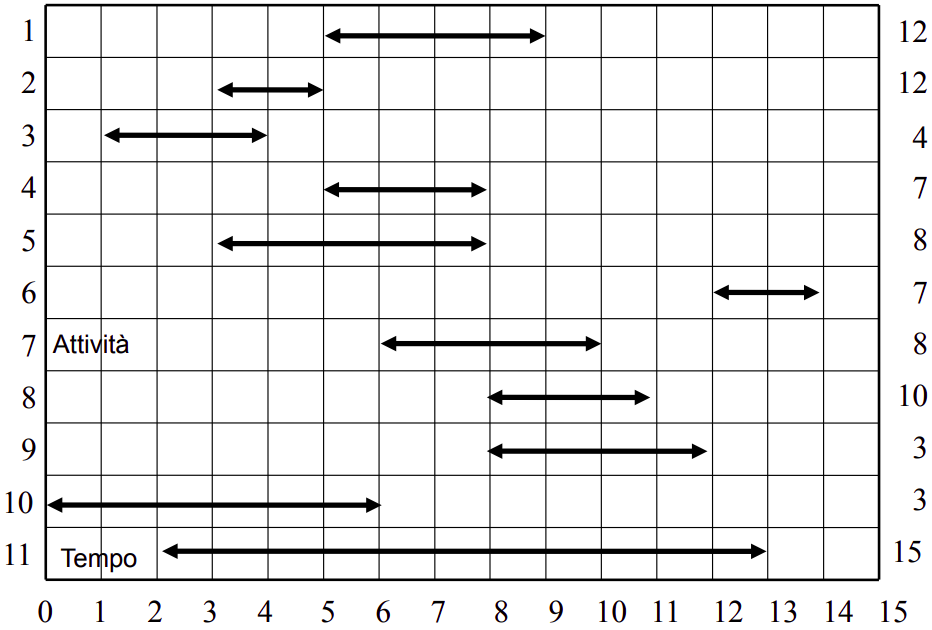
\includegraphics[width=0.8\textwidth]{intervalli.png}
    \end{figure*}\noindent
    Siccome non possono esserci sovrapposizioni, se l'hotel decidesse di
    concedere la sala al cliente 6, non potrebbe concederla al cliente 11
    perché i due intervalli di tempo si intersecherebbero.

    Il problema con questa disposizione è che preso un intervallo, per capire
    quali altri intervalli possono ancora essere considerati, siamo costretti ad
    analizzarli tutti. Tuttavia, in una situazione come questa può essere
    conveniente eseguire una pre-elaborazione dei dati, per esempio, potremmo
    ordinare gli intervalli per estremi di fine non decrescenti.

    \begin{figure*}[ht!]
        \centering
        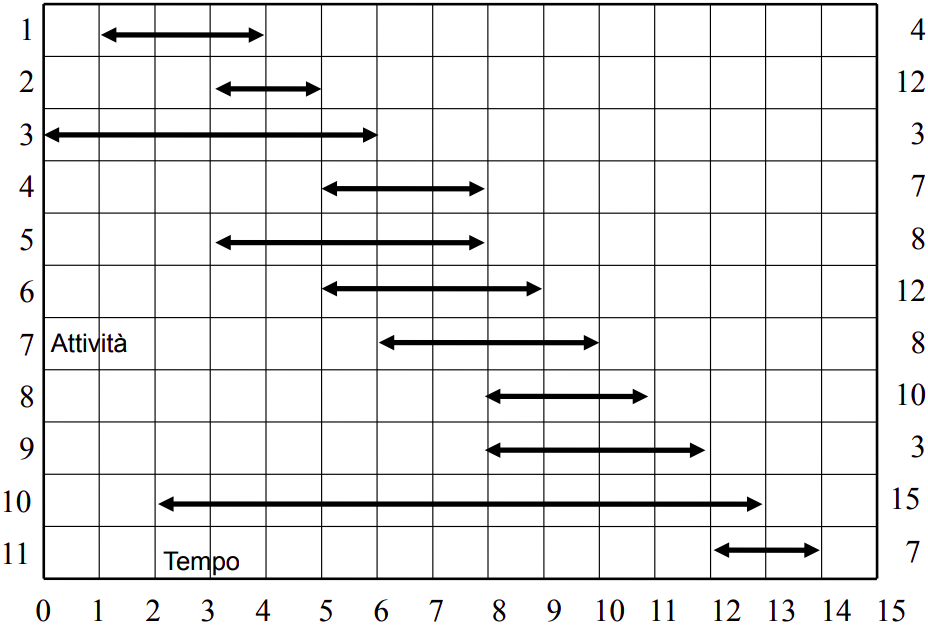
\includegraphics[width=0.8\textwidth]{intervalli-ordinati.png}
    \end{figure*}\noindent
    Ora, per decidere se tenere o meno l'ultimo intervallo, possiamo procedere
    come abbiamo fatto negli esempi precedenti, cioè considerando una qualche
    tabella $DP$ associata all'intervallo di tempo che si conclude nell'istante
    in cui inizia l'intervallo considerato.

    \bigskip\noindent
    Per rispondere al quesito originale, l'hotel può massimizzare
    i profitti concedendo la sala ai clienti: $2$, $4$, $8$ e $11$.
\end{eg}

\noindent
Chiarita la necessità di effettuare una pre-elaborazione, dobbiamo decidere in
che modo trattare i dati. L'idea già citata è quella di ordinare gli intervalli
per estremi di fine non decrescenti, cioè ordinarli in modo che $b_1\leq
\dots\leq b_n$. A questo punto, definiamo una tabella $DP$ tale che $DP[i]$
contenga il massimo profitto realizzabile con i primi $i$ intervalli:
\[DP[i]=\begin{cases}
    0 & i=0\\
    \max\left(DP[i-1], \max\left\{DP[j]+w_[i]:j<i\wedge b_j\leq a_i\right\}\right)
    & i>0
\end{cases}\]
Con questa soluzione, cercare l'indice $j$ costa $O(n)$ perché partendo
dall'intervallo $i$ è necessario scandire tutti gli altri. Poiché quest'operazione
dev'essere ripetuto per ogni intervallo, il costo finale è $O(n^2)$.

\bigskip\noindent
È possibile trovare una pre-elaborazione migliore?

Potremmo provare a pre-calcolare il predecessore $pred_i=j$ di $i$ tale che
$j$ sia il massimo valore minore di $i$ per cui $b_j\leq a_i$. Se non esiste un
tale valore, consideriamo $pred_i=0$. Noto il predecessore, la definizione di
$DP$ diventa:
\[DP[i]=\begin{cases}
    0 & i=0\\
    \max\left(DP[i-1],DP[pred_i]+w[i]\right) & i>0
\end{cases}\]
\begin{note}
    È possibile escludere un intervallo $i$, se sceglierne un altro $j$ con
    stesso tempo di fine, ma tempo di inizio precedente, ha un valore
    $DP[j]>DP[i]$.
\end{note}\noindent
Un modo per calcolare i predecessori è il seguente:

\begin{minicode}{Funzione per il calcolo dei predecessori}
\ind\bc{int}[]  computePredecessors(\bc{int}[] a, \bc{int}[] b, \bc{int} n)\\
    \bc{int}[] pred = new \bc{int}[0\dots n]\\
    pred[0] = 0\\
    \indf for (i = 1 to n) do\\
        j = i - 1\\
        \indff while (j > 0 and b[j] > a[i]) do\\
            j = j - 1\\
        \indff pred[i] = j\\
    \indf return pred
\end{minicode}\noindent
Il costo di questa funzione rimane $O(n^2)$, ma esistono delle implementazioni
di \emph{complessità} $O(n\log n)$.

\begin{minicode}{Implementazione della soluzione}
\ind\bc{SET} maxInterval(\bc{int}[] a, \bc{int}[] b, \bc{int}[] w, \bc{int} n)\\
    \com{\{ Ordina gli intervalli per estremi di fine non decrescenti \}}
    \bc{int}[] pred = computePredecessors(a, b, n)\\
    \bc{int}[] DP = new \bc{int}[0\dots n]\\
    DP[0] = 0\\
    \indf for (i = 1 to n) do\hfill\com{Riempimento tabelle delle soluzioni}
        DP[i] = max(DP[i - 1], DP[pred[i]] + w[i])\\
    \indf\bc{int} i = n\\
    \indf\bc{SET} S = Set()\\
\end{minicode}
\begin{codecont}
    \indent while (i > 0) do\hfill\com{Ricostruzione della soluzione}
        \indf if (DP[i - 1] > DP[pred[i]] + w[i]) do\\
            \indff i = i - 1\\
    \rmindent\indent else\\
            \indff S.insert(i)\\
            \indff i = pred[i]\\
    \ind return S
\end{codecont}

\paragraph{Complessità}
La \emph{complessità} dell'intero algoritmo è $O(n\log n)$ in quanto paghiamo
$O(n\log n)$ per ordinare gli intervalli e calcolare i predecessori, mentre per
popolare la tabella e ricostruire la soluzione paghiamo $\Theta(n)$.